\documentclass{article}
\usepackage[utf8]{inputenc}
\usepackage{booktabs}
\usepackage{graphicx}
\usepackage{float}
\usepackage{geometry}
\geometry{a4paper, margin=1in}
\begin{document}

\title{Resultados de Simulación RCWA - Comparativa de Geometrías y Rotaciones}
\author{Sergio Montoya (Reporte Automatizado)}
\date{\today}
\maketitle

El presente reporte detalla los \textit{Photonic Bandgaps} y la estructura de bandas detectados en simulaciones RCWA, evaluando tanto barridos de vector de onda ($k_x$) como de rotación (twist).
Se asume un umbral de transmisión del 12\% para el cálculo de bandgaps, mitigando los efectos de fuga numérica por bajos órdenes de difracción.
\clearpage
\input{materiales/PMMA Dopping + FeCl3 thickness 200}
\section{PMMA Dopping + I2 thickness 100}
\subsection*{Material ID: Dopping: 0}
\textbf{Constante Dieléctrica ($\epsilon_{total}$):} 2.57 \\[0.5em]
\begin{table}[h!]
\centering
\begin{tabular}{lcc}
\toprule
\textbf{Métrica} & \textbf{Lámina (Plate)} & \textbf{Cilindros (Rod)} \\
\midrule
Bandgaps ($k_x$) & Ninguno & Ninguno \\
Resonancias ($k_x$) & 36 & 36 \\
\midrule
Bandgaps (Rotación) & Ninguno & Ninguno \\
Resonancias (Rotación) & 33 & 33 \\
\bottomrule
\end{tabular}
\end{table}
\begin{figure}[H]
\centering
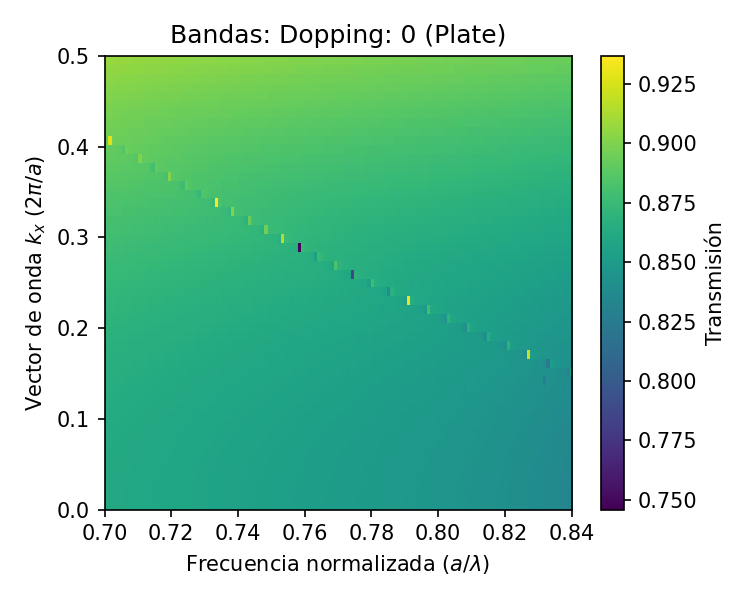
\includegraphics[width=0.48\textwidth]{figures/Dopping: 0_plate.png}
\hfill
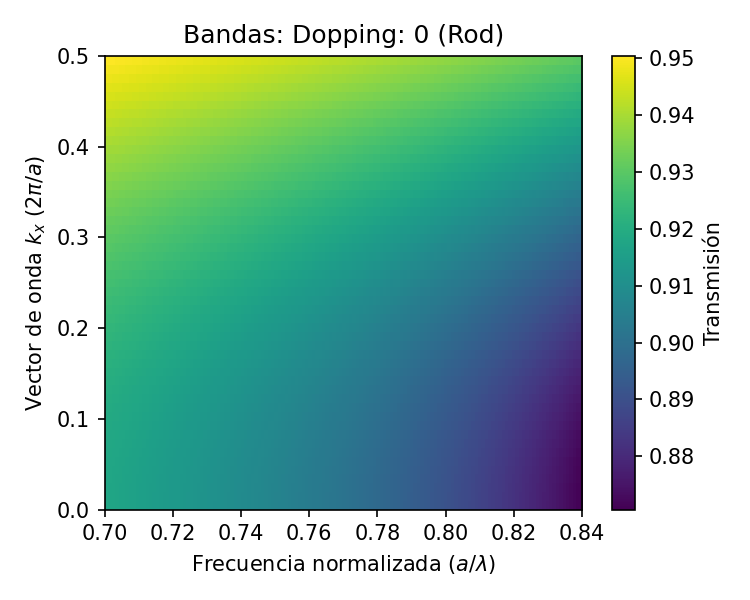
\includegraphics[width=0.48\textwidth]{figures/Dopping: 0_rod.png}
\caption{Estructuras de bandas fotónicas ($k_x$) para Dopping: 0. Izquierda: Lámina. Derecha: Cilindros.}
\end{figure}
\vspace{1em}
\begin{figure}[H]
\centering
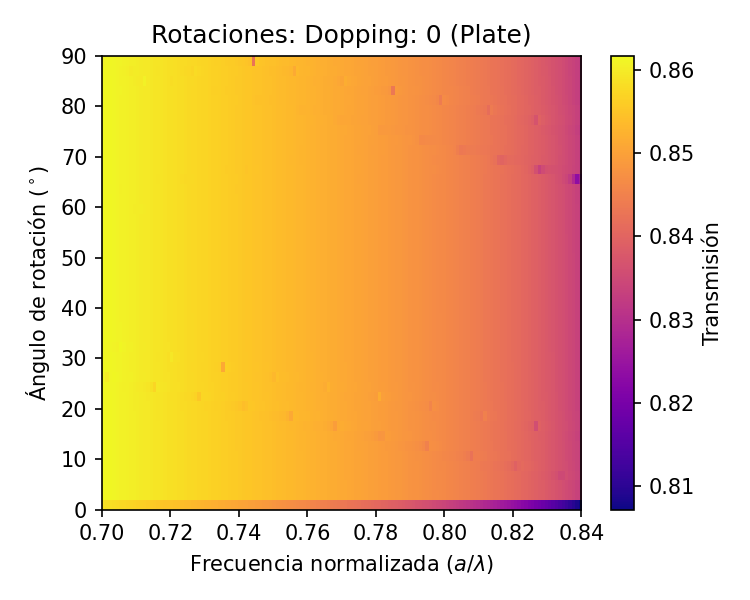
\includegraphics[width=0.48\textwidth]{figures/Dopping: 0_plate_rangle.png}
\hfill
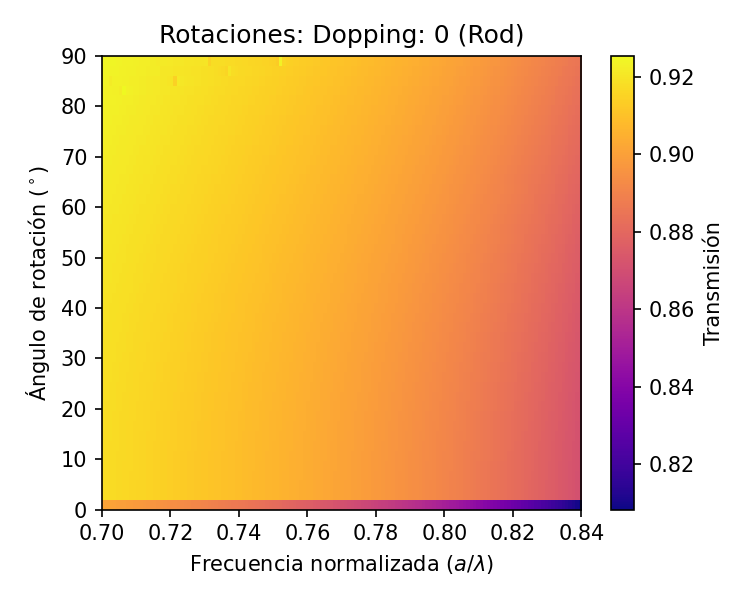
\includegraphics[width=0.48\textwidth]{figures/Dopping: 0_rod_rangle.png}
\caption{Mapas de transmisión por rotación (twist) para Dopping: 0. Izquierda: Lámina. Derecha: Cilindros.}
\end{figure}
\vspace{1em}
\hrule
\vspace{1em}
\subsection*{Material ID: Dopping: 2}
\textbf{Constante Dieléctrica ($\epsilon_{total}$):} 2.67 \\[0.5em]
\begin{table}[h!]
\centering
\begin{tabular}{lcc}
\toprule
\textbf{Métrica} & \textbf{Lámina (Plate)} & \textbf{Cilindros (Rod)} \\
\midrule
Bandgaps ($k_x$) & Ninguno & Ninguno \\
Resonancias ($k_x$) & 36 & 36 \\
\midrule
Bandgaps (Rotación) & Ninguno & Ninguno \\
Resonancias (Rotación) & 33 & 33 \\
\bottomrule
\end{tabular}
\end{table}
\begin{figure}[H]
\centering
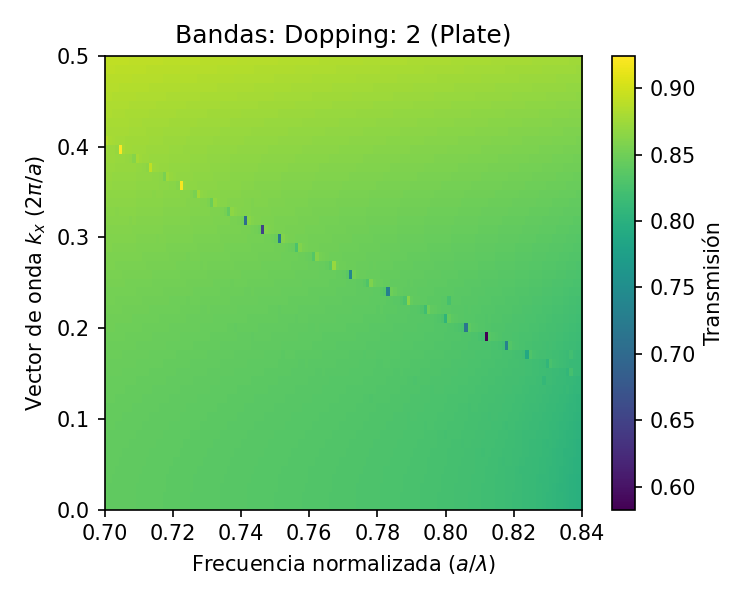
\includegraphics[width=0.48\textwidth]{figures/Dopping: 2_plate.png}
\hfill
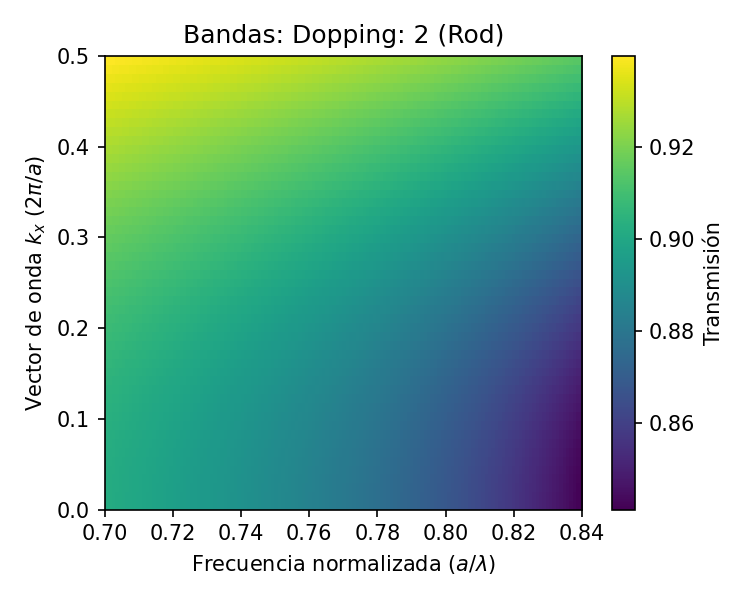
\includegraphics[width=0.48\textwidth]{figures/Dopping: 2_rod.png}
\caption{Estructuras de bandas fotónicas ($k_x$) para Dopping: 2. Izquierda: Lámina. Derecha: Cilindros.}
\end{figure}
\vspace{1em}
\begin{figure}[H]
\centering
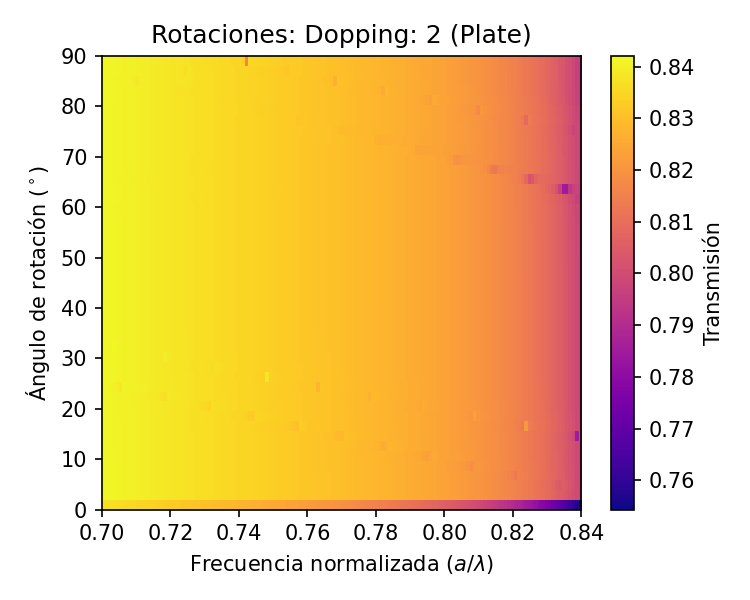
\includegraphics[width=0.48\textwidth]{figures/Dopping: 2_plate_rangle.png}
\hfill
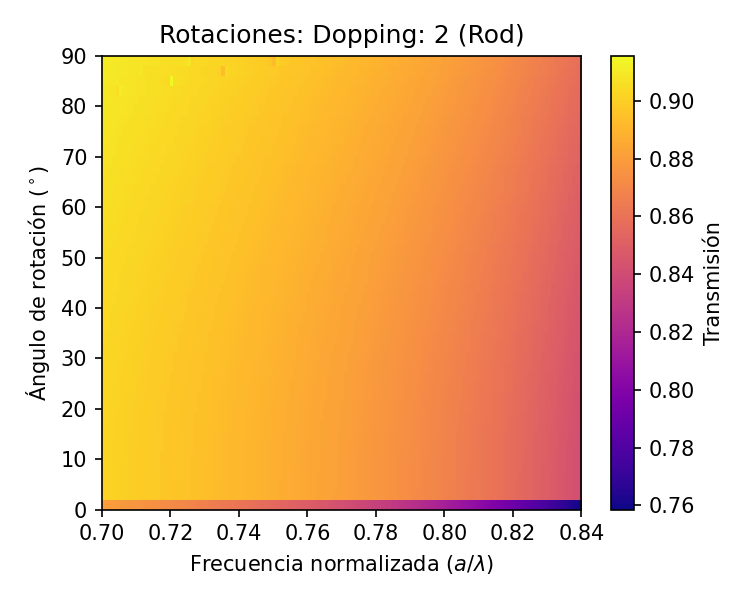
\includegraphics[width=0.48\textwidth]{figures/Dopping: 2_rod_rangle.png}
\caption{Mapas de transmisión por rotación (twist) para Dopping: 2. Izquierda: Lámina. Derecha: Cilindros.}
\end{figure}
\vspace{1em}
\hrule
\vspace{1em}
\subsection*{Material ID: Dopping: 4}
\textbf{Constante Dieléctrica ($\epsilon_{total}$):} 2.80 \\[0.5em]
\begin{table}[h!]
\centering
\begin{tabular}{lcc}
\toprule
\textbf{Métrica} & \textbf{Lámina (Plate)} & \textbf{Cilindros (Rod)} \\
\midrule
Bandgaps ($k_x$) & Ninguno & Ninguno \\
Resonancias ($k_x$) & 36 & 36 \\
\midrule
Bandgaps (Rotación) & Ninguno & Ninguno \\
Resonancias (Rotación) & 33 & 33 \\
\bottomrule
\end{tabular}
\end{table}
\begin{figure}[H]
\centering
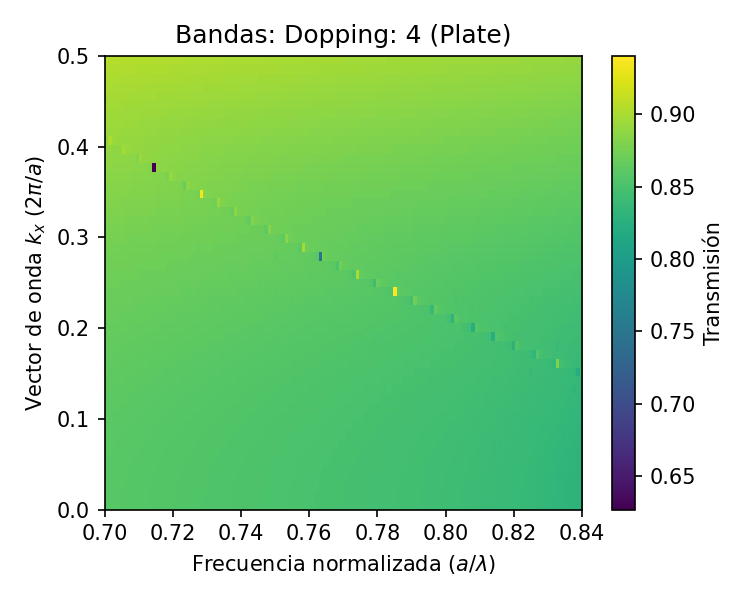
\includegraphics[width=0.48\textwidth]{figures/Dopping: 4_plate.png}
\hfill
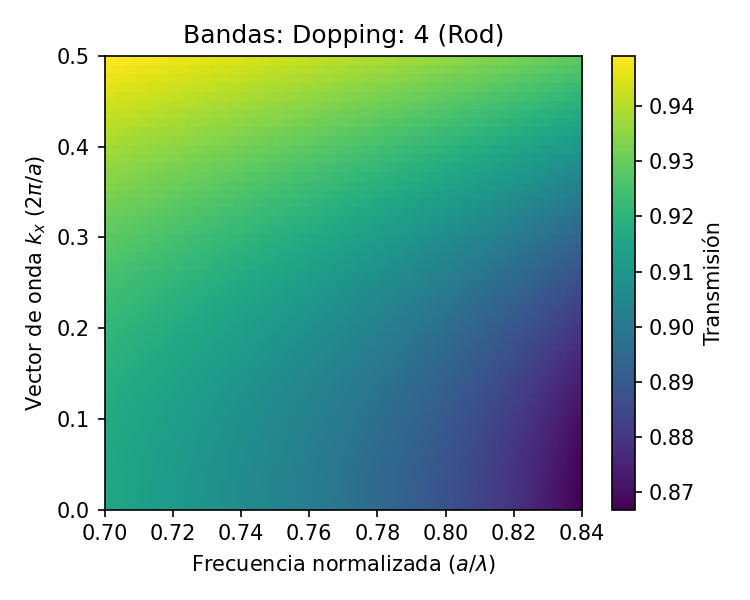
\includegraphics[width=0.48\textwidth]{figures/Dopping: 4_rod.png}
\caption{Estructuras de bandas fotónicas ($k_x$) para Dopping: 4. Izquierda: Lámina. Derecha: Cilindros.}
\end{figure}
\vspace{1em}
\begin{figure}[H]
\centering
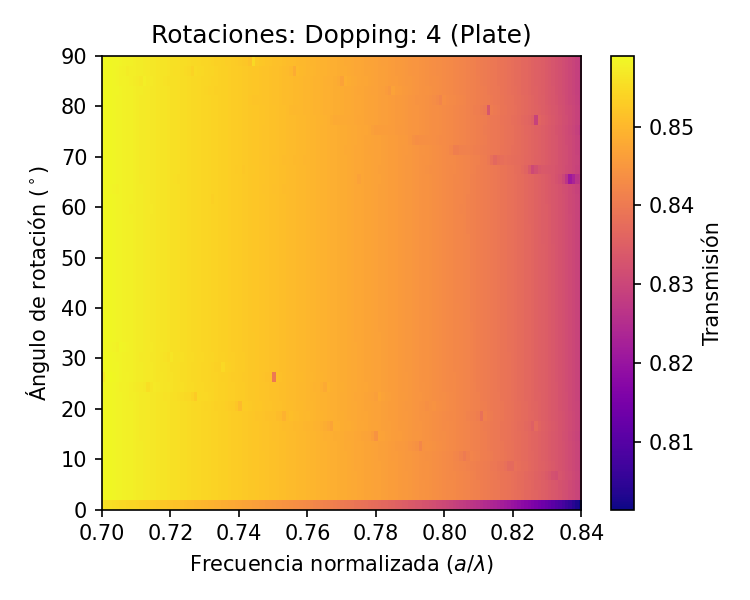
\includegraphics[width=0.48\textwidth]{figures/Dopping: 4_plate_rangle.png}
\hfill
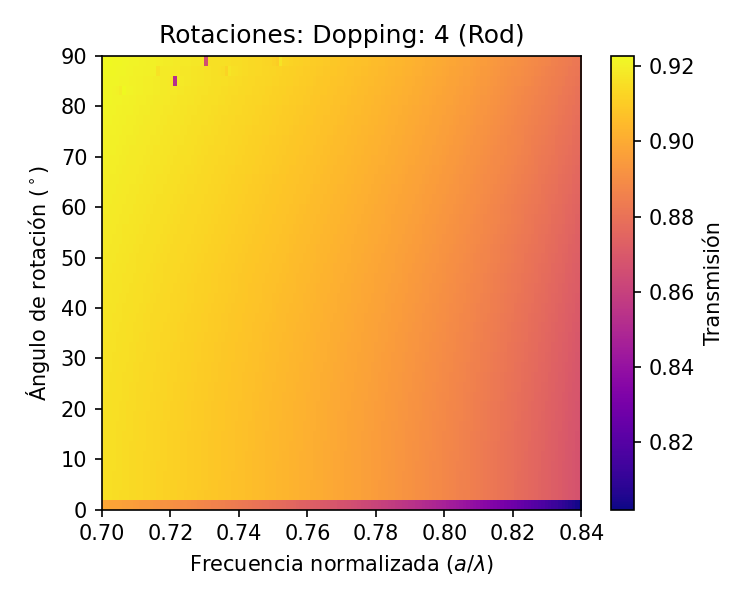
\includegraphics[width=0.48\textwidth]{figures/Dopping: 4_rod_rangle.png}
\caption{Mapas de transmisión por rotación (twist) para Dopping: 4. Izquierda: Lámina. Derecha: Cilindros.}
\end{figure}
\vspace{1em}
\hrule
\vspace{1em}
\subsection*{Material ID: Dopping: 6}
\textbf{Constante Dieléctrica ($\epsilon_{total}$):} 2.86 \\[0.5em]
\begin{table}[h!]
\centering
\begin{tabular}{lcc}
\toprule
\textbf{Métrica} & \textbf{Lámina (Plate)} & \textbf{Cilindros (Rod)} \\
\midrule
Bandgaps ($k_x$) & Ninguno & Ninguno \\
Resonancias ($k_x$) & 36 & 36 \\
\midrule
Bandgaps (Rotación) & Ninguno & Ninguno \\
Resonancias (Rotación) & 33 & 33 \\
\bottomrule
\end{tabular}
\end{table}
\begin{figure}[H]
\centering
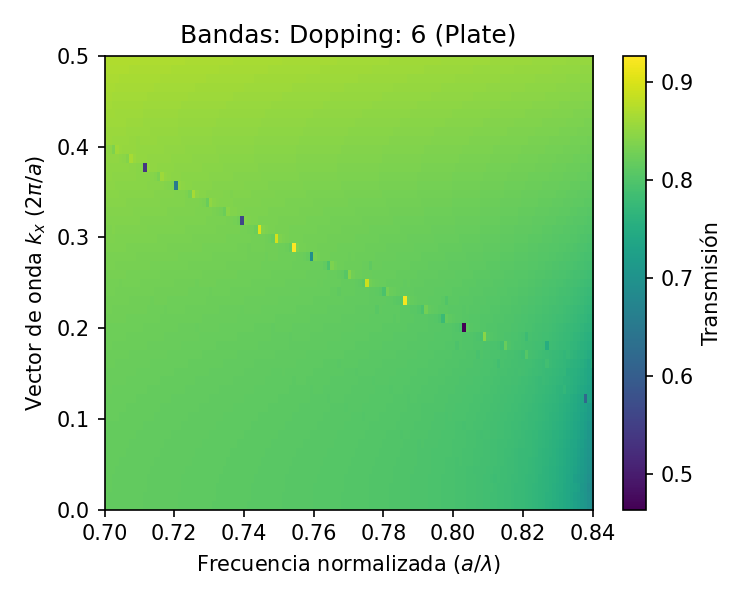
\includegraphics[width=0.48\textwidth]{figures/Dopping: 6_plate.png}
\hfill
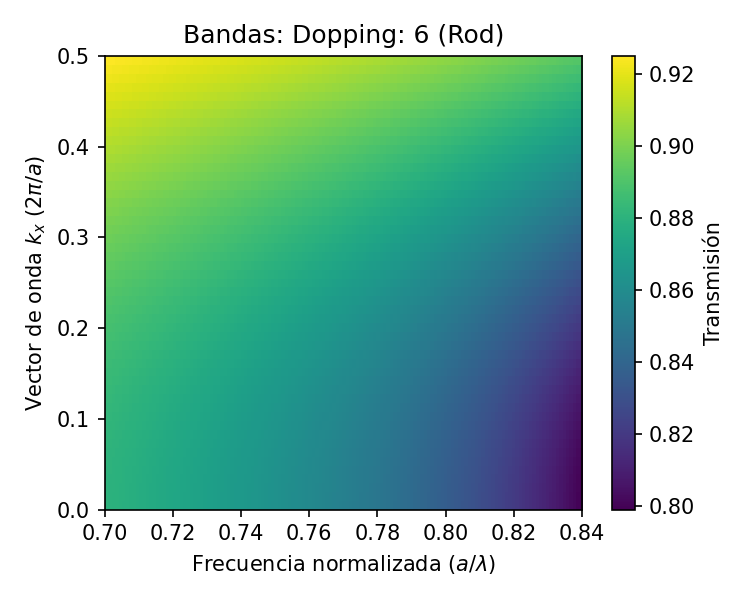
\includegraphics[width=0.48\textwidth]{figures/Dopping: 6_rod.png}
\caption{Estructuras de bandas fotónicas ($k_x$) para Dopping: 6. Izquierda: Lámina. Derecha: Cilindros.}
\end{figure}
\vspace{1em}
\begin{figure}[H]
\centering
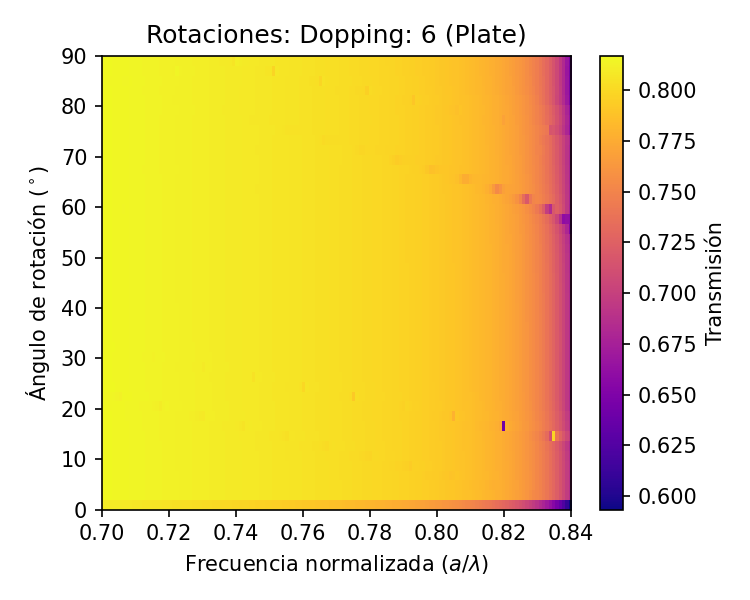
\includegraphics[width=0.48\textwidth]{figures/Dopping: 6_plate_rangle.png}
\hfill
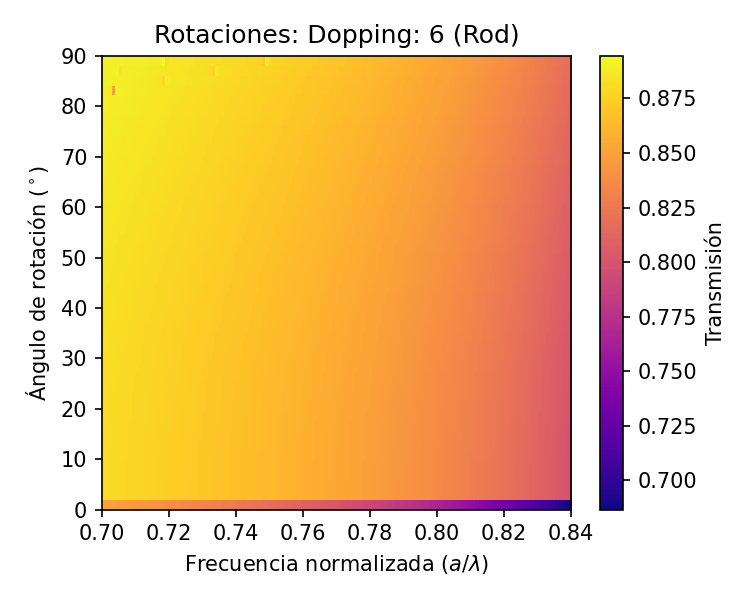
\includegraphics[width=0.48\textwidth]{figures/Dopping: 6_rod_rangle.png}
\caption{Mapas de transmisión por rotación (twist) para Dopping: 6. Izquierda: Lámina. Derecha: Cilindros.}
\end{figure}
\vspace{1em}
\hrule
\vspace{1em}
\subsection*{Material ID: Dopping: 8}
\textbf{Constante Dieléctrica ($\epsilon_{total}$):} 2.88 \\[0.5em]
\begin{table}[h!]
\centering
\begin{tabular}{lcc}
\toprule
\textbf{Métrica} & \textbf{Lámina (Plate)} & \textbf{Cilindros (Rod)} \\
\midrule
Bandgaps ($k_x$) & Ninguno & Ninguno \\
Resonancias ($k_x$) & 36 & 36 \\
\midrule
Bandgaps (Rotación) & Ninguno & Ninguno \\
Resonancias (Rotación) & 33 & 33 \\
\bottomrule
\end{tabular}
\end{table}
\begin{figure}[H]
\centering
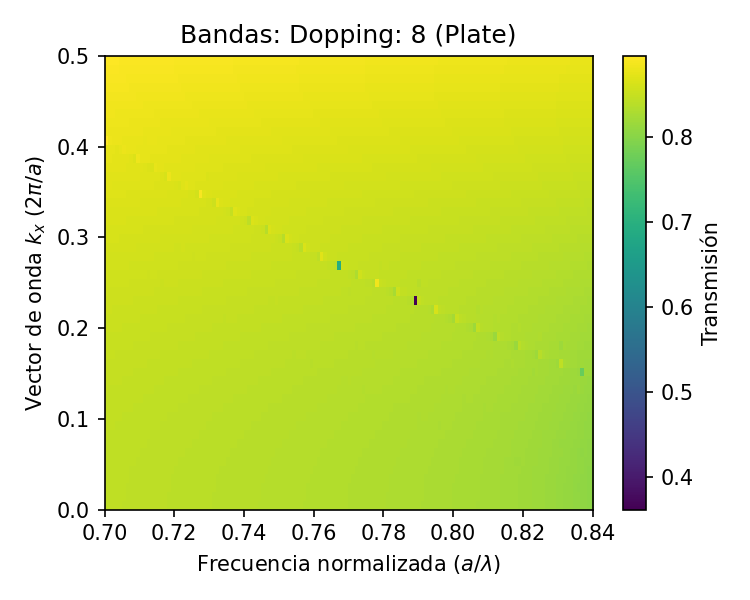
\includegraphics[width=0.48\textwidth]{figures/Dopping: 8_plate.png}
\hfill
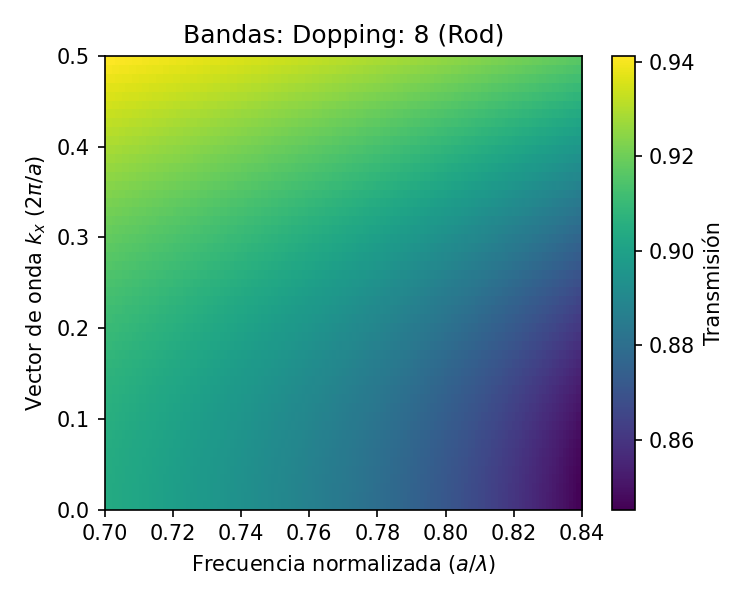
\includegraphics[width=0.48\textwidth]{figures/Dopping: 8_rod.png}
\caption{Estructuras de bandas fotónicas ($k_x$) para Dopping: 8. Izquierda: Lámina. Derecha: Cilindros.}
\end{figure}
\vspace{1em}
\begin{figure}[H]
\centering
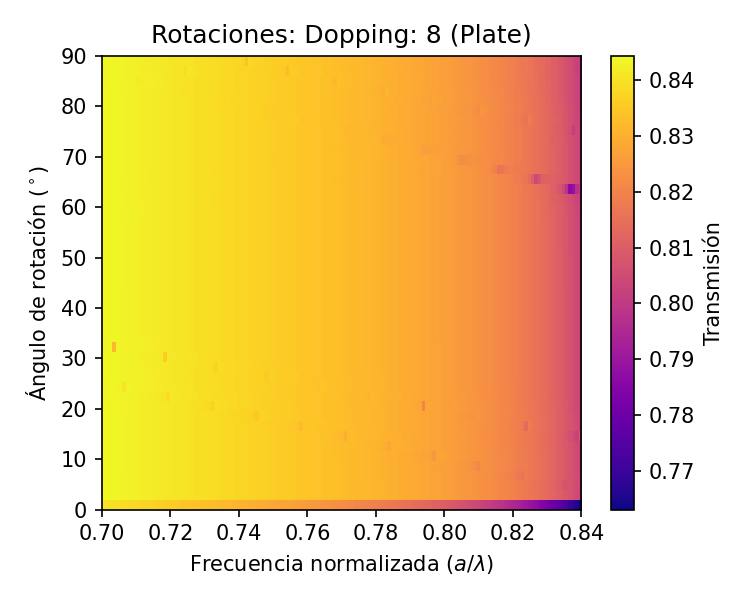
\includegraphics[width=0.48\textwidth]{figures/Dopping: 8_plate_rangle.png}
\hfill
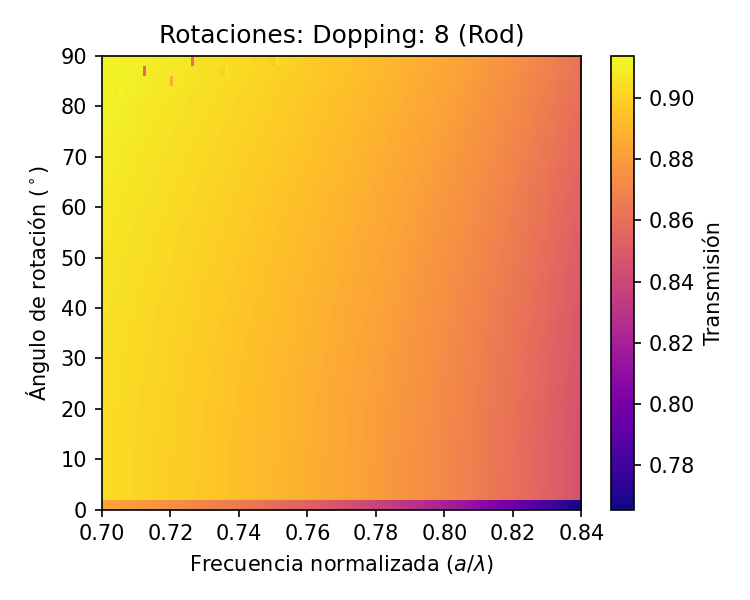
\includegraphics[width=0.48\textwidth]{figures/Dopping: 8_rod_rangle.png}
\caption{Mapas de transmisión por rotación (twist) para Dopping: 8. Izquierda: Lámina. Derecha: Cilindros.}
\end{figure}
\vspace{1em}
\hrule
\vspace{1em}
\clearpage
\section{PMMA Dopping + benzoic acid thickness 100}
\subsection*{Material ID: Dopping: 0}
\textbf{Constante Dieléctrica ($\epsilon_{total}$):} 2.52 \\[0.5em]
\begin{table}[h!]
\centering
\begin{tabular}{lcc}
\toprule
\textbf{Métrica} & \textbf{Lámina (Plate)} & \textbf{Cilindros (Rod)} \\
\midrule
Bandgaps ($k_x$) & Ninguno & Ninguno \\
Resonancias ($k_x$) & 36 & 36 \\
\midrule
Bandgaps (Rotación) & Ninguno & Ninguno \\
Resonancias (Rotación) & 33 & 33 \\
\bottomrule
\end{tabular}
\end{table}
\begin{figure}[H]
\centering
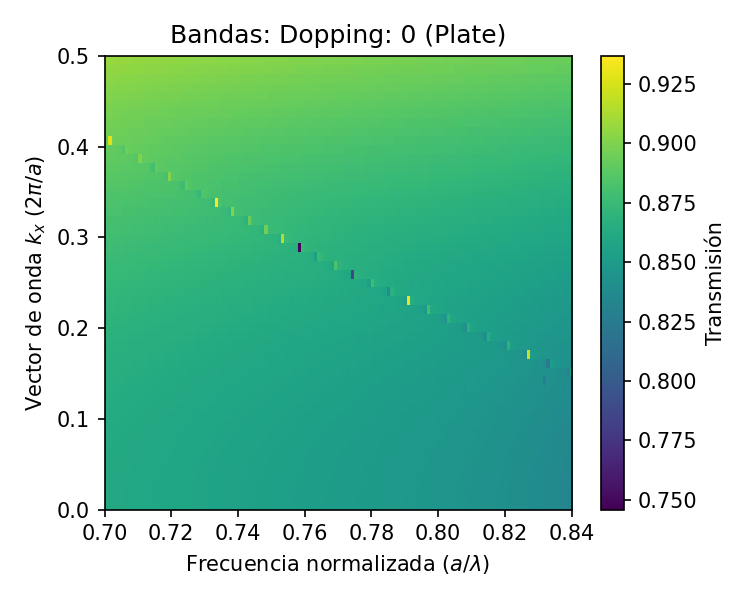
\includegraphics[width=0.48\textwidth]{figures/Dopping: 0_plate.png}
\hfill
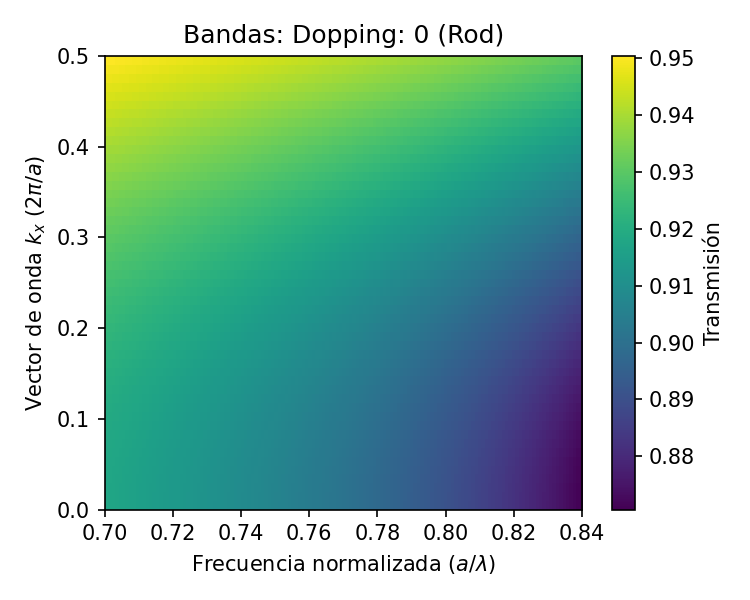
\includegraphics[width=0.48\textwidth]{figures/Dopping: 0_rod.png}
\caption{Estructuras de bandas fotónicas ($k_x$) para Dopping: 0. Izquierda: Lámina. Derecha: Cilindros.}
\end{figure}
\vspace{1em}
\begin{figure}[H]
\centering
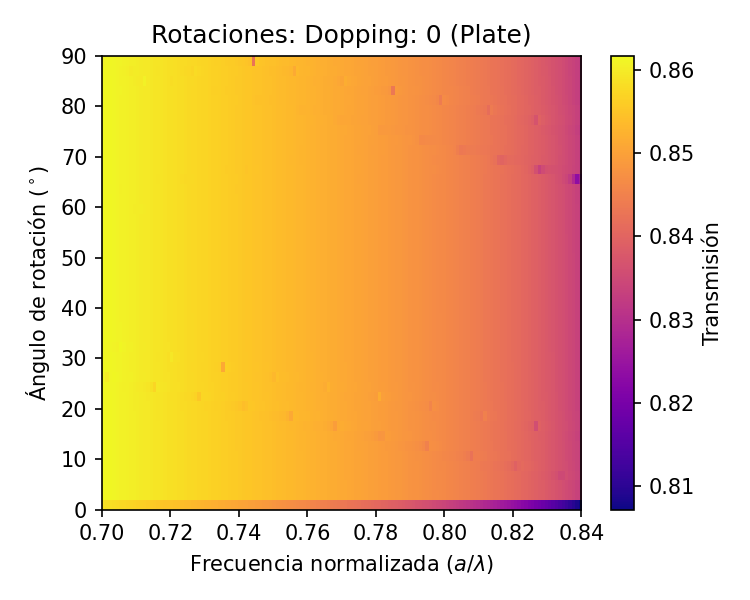
\includegraphics[width=0.48\textwidth]{figures/Dopping: 0_plate_rangle.png}
\hfill
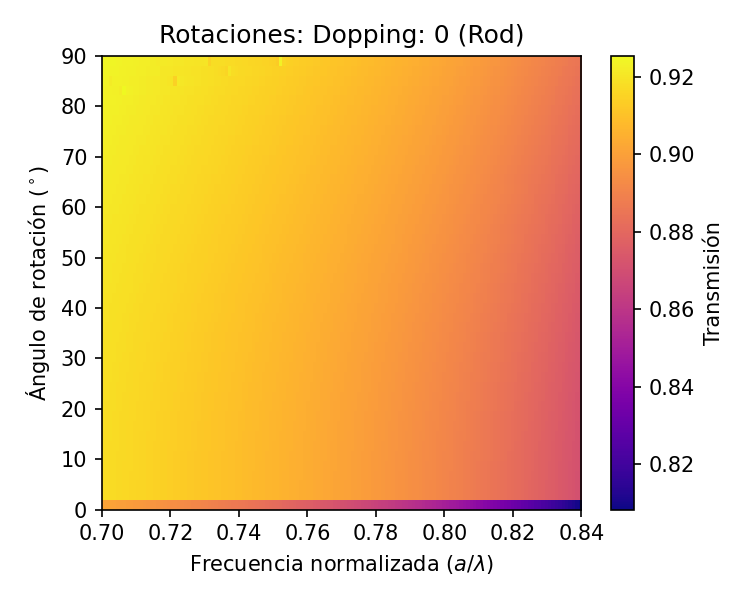
\includegraphics[width=0.48\textwidth]{figures/Dopping: 0_rod_rangle.png}
\caption{Mapas de transmisión por rotación (twist) para Dopping: 0. Izquierda: Lámina. Derecha: Cilindros.}
\end{figure}
\vspace{1em}
\hrule
\vspace{1em}
\subsection*{Material ID: Dopping: 12}
\textbf{Constante Dieléctrica ($\epsilon_{total}$):} 2.78 \\[0.5em]
\begin{table}[h!]
\centering
\begin{tabular}{lcc}
\toprule
\textbf{Métrica} & \textbf{Lámina (Plate)} & \textbf{Cilindros (Rod)} \\
\midrule
Bandgaps ($k_x$) & Ninguno & Ninguno \\
Resonancias ($k_x$) & 36 & 36 \\
\midrule
Bandgaps (Rotación) & Ninguno & Ninguno \\
Resonancias (Rotación) & 33 & 33 \\
\bottomrule
\end{tabular}
\end{table}
\begin{figure}[H]
\centering
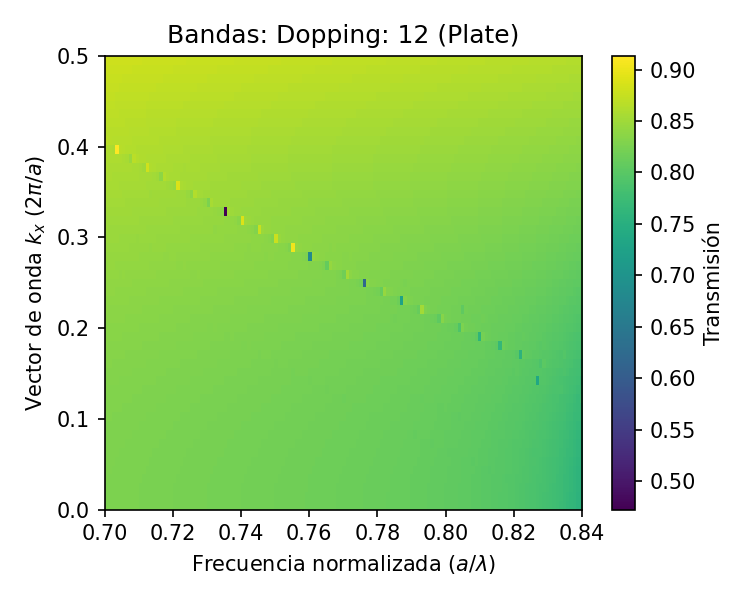
\includegraphics[width=0.48\textwidth]{figures/Dopping: 12_plate.png}
\hfill
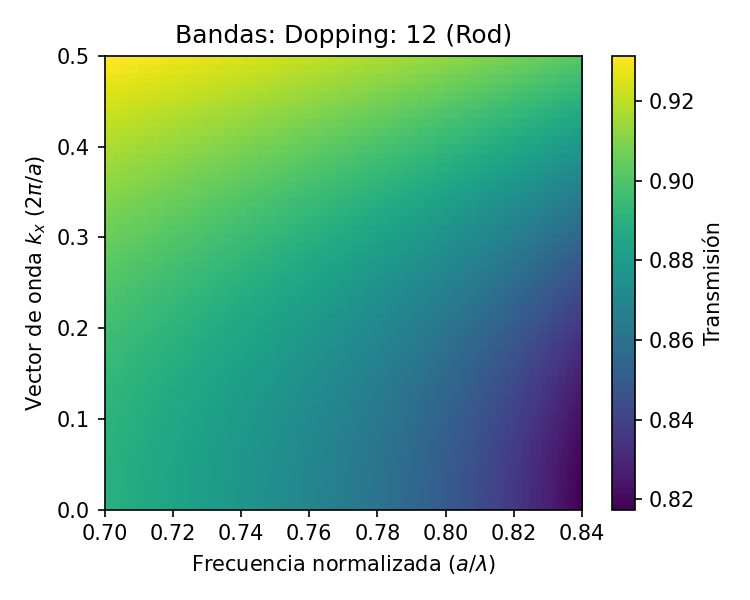
\includegraphics[width=0.48\textwidth]{figures/Dopping: 12_rod.png}
\caption{Estructuras de bandas fotónicas ($k_x$) para Dopping: 12. Izquierda: Lámina. Derecha: Cilindros.}
\end{figure}
\vspace{1em}
\begin{figure}[H]
\centering
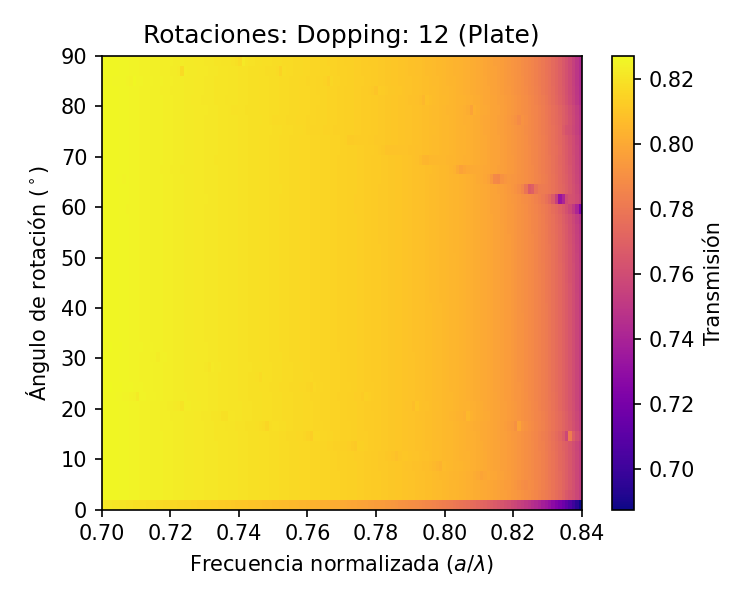
\includegraphics[width=0.48\textwidth]{figures/Dopping: 12_plate_rangle.png}
\hfill
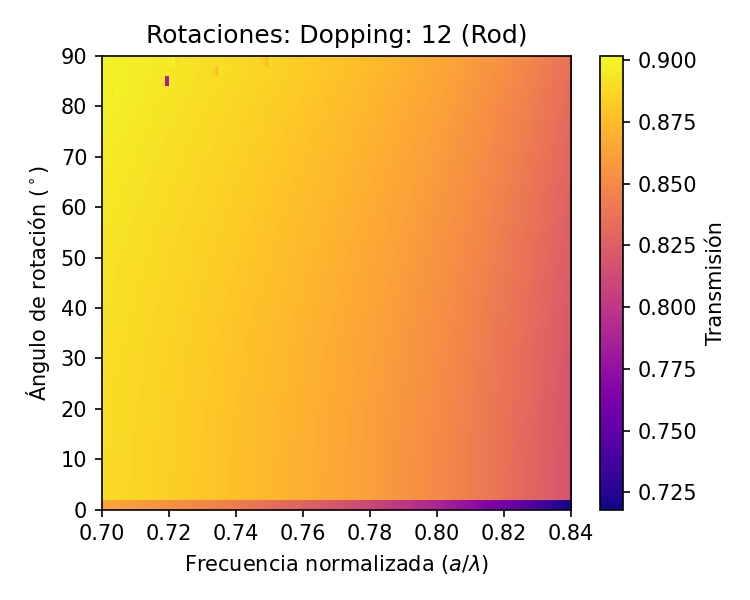
\includegraphics[width=0.48\textwidth]{figures/Dopping: 12_rod_rangle.png}
\caption{Mapas de transmisión por rotación (twist) para Dopping: 12. Izquierda: Lámina. Derecha: Cilindros.}
\end{figure}
\vspace{1em}
\hrule
\vspace{1em}
\subsection*{Material ID: Dopping: 16}
\textbf{Constante Dieléctrica ($\epsilon_{total}$):} 2.60 \\[0.5em]
\begin{table}[h!]
\centering
\begin{tabular}{lcc}
\toprule
\textbf{Métrica} & \textbf{Lámina (Plate)} & \textbf{Cilindros (Rod)} \\
\midrule
Bandgaps ($k_x$) & Ninguno & Ninguno \\
Resonancias ($k_x$) & 36 & 36 \\
\midrule
Bandgaps (Rotación) & Ninguno & Ninguno \\
Resonancias (Rotación) & 33 & 33 \\
\bottomrule
\end{tabular}
\end{table}
\begin{figure}[H]
\centering
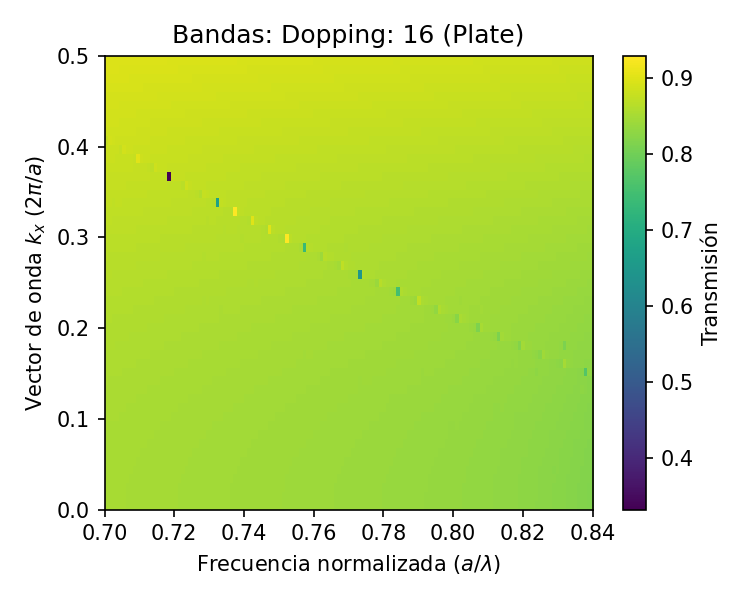
\includegraphics[width=0.48\textwidth]{figures/Dopping: 16_plate.png}
\hfill
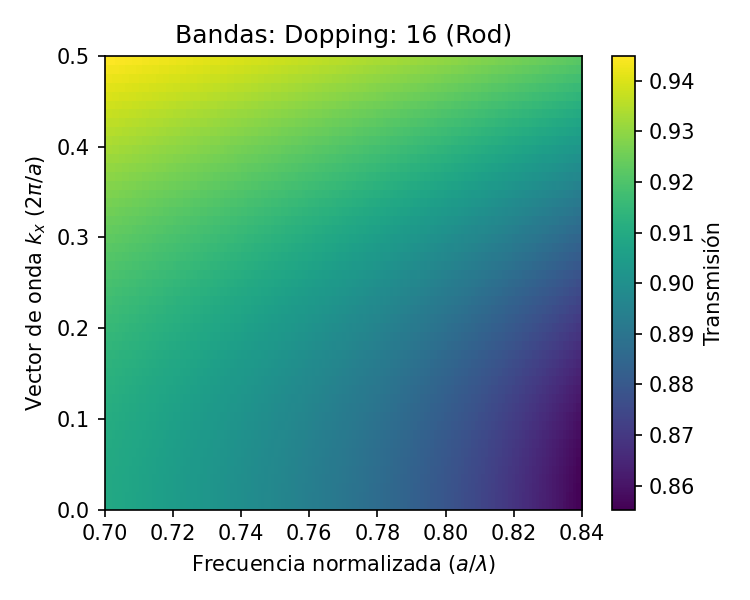
\includegraphics[width=0.48\textwidth]{figures/Dopping: 16_rod.png}
\caption{Estructuras de bandas fotónicas ($k_x$) para Dopping: 16. Izquierda: Lámina. Derecha: Cilindros.}
\end{figure}
\vspace{1em}
\begin{figure}[H]
\centering
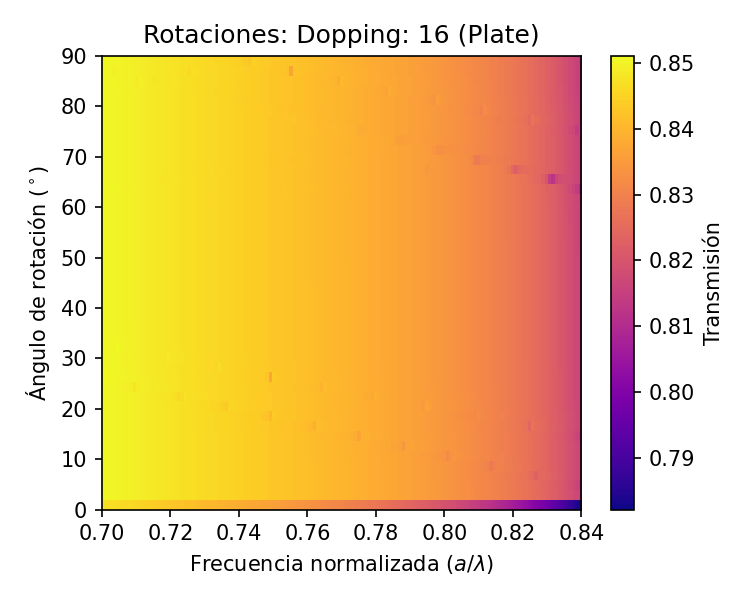
\includegraphics[width=0.48\textwidth]{figures/Dopping: 16_plate_rangle.png}
\hfill
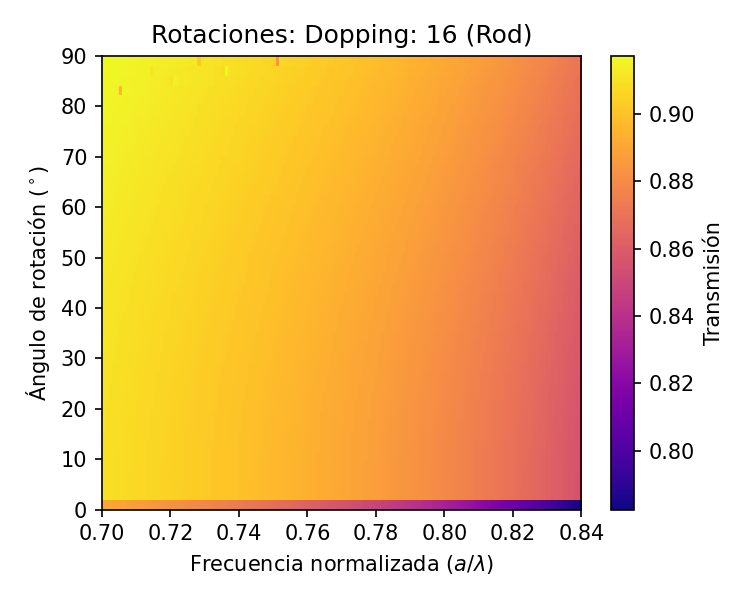
\includegraphics[width=0.48\textwidth]{figures/Dopping: 16_rod_rangle.png}
\caption{Mapas de transmisión por rotación (twist) para Dopping: 16. Izquierda: Lámina. Derecha: Cilindros.}
\end{figure}
\vspace{1em}
\hrule
\vspace{1em}
\subsection*{Material ID: Dopping: 20}
\textbf{Constante Dieléctrica ($\epsilon_{total}$):} 3.00 \\[0.5em]
\begin{table}[h!]
\centering
\begin{tabular}{lcc}
\toprule
\textbf{Métrica} & \textbf{Lámina (Plate)} & \textbf{Cilindros (Rod)} \\
\midrule
Bandgaps ($k_x$) & Ninguno & Ninguno \\
Resonancias ($k_x$) & 36 & 36 \\
\midrule
Bandgaps (Rotación) & Ninguno & Ninguno \\
Resonancias (Rotación) & 33 & 33 \\
\bottomrule
\end{tabular}
\end{table}
\begin{figure}[H]
\centering
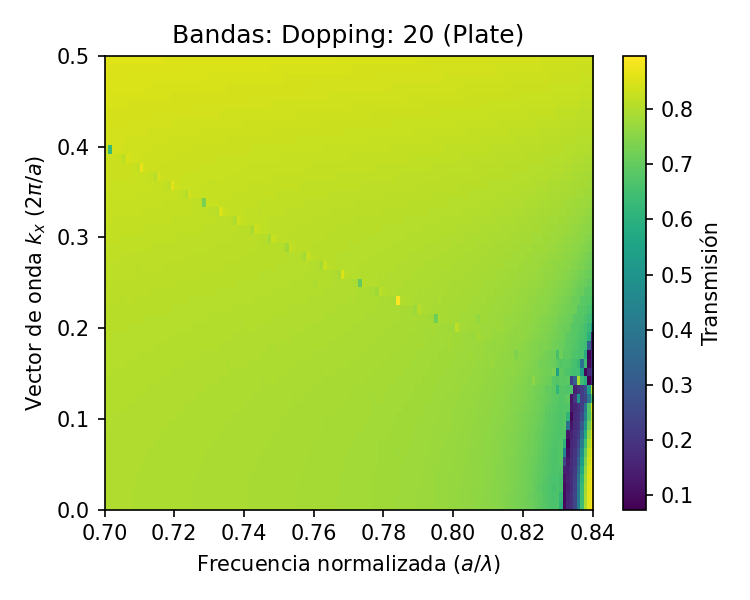
\includegraphics[width=0.48\textwidth]{figures/Dopping: 20_plate.png}
\hfill
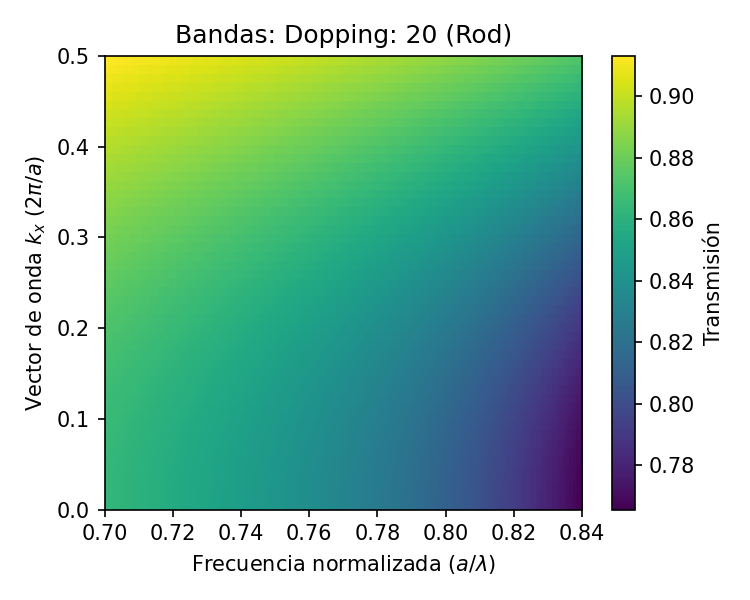
\includegraphics[width=0.48\textwidth]{figures/Dopping: 20_rod.png}
\caption{Estructuras de bandas fotónicas ($k_x$) para Dopping: 20. Izquierda: Lámina. Derecha: Cilindros.}
\end{figure}
\vspace{1em}
\begin{figure}[H]
\centering
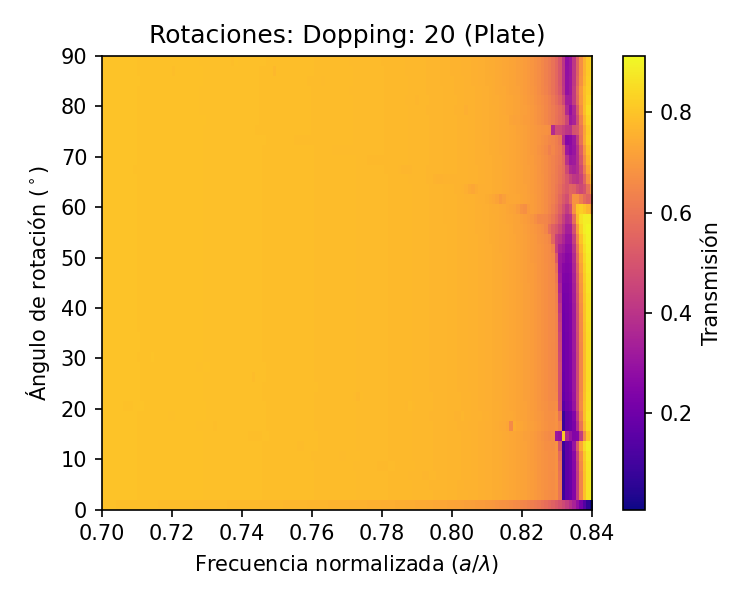
\includegraphics[width=0.48\textwidth]{figures/Dopping: 20_plate_rangle.png}
\hfill
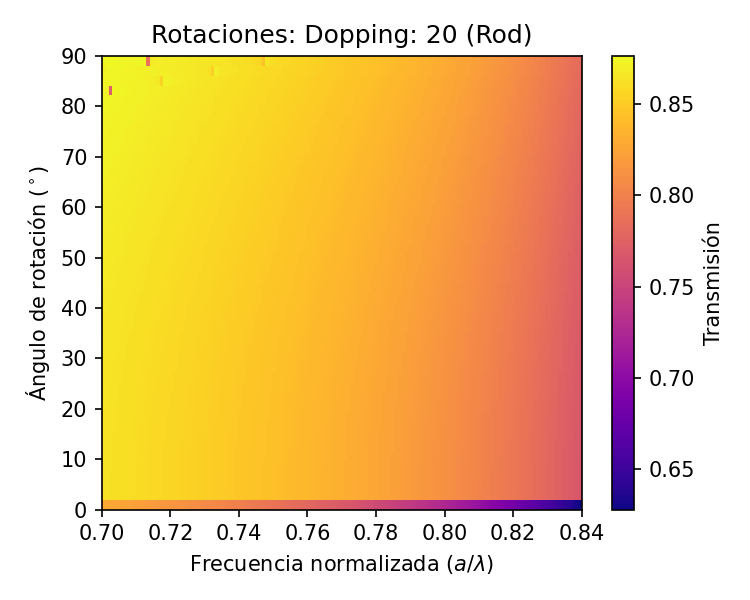
\includegraphics[width=0.48\textwidth]{figures/Dopping: 20_rod_rangle.png}
\caption{Mapas de transmisión por rotación (twist) para Dopping: 20. Izquierda: Lámina. Derecha: Cilindros.}
\end{figure}
\vspace{1em}
\hrule
\vspace{1em}
\subsection*{Material ID: Dopping: 4}
\textbf{Constante Dieléctrica ($\epsilon_{total}$):} 2.54 \\[0.5em]
\begin{table}[h!]
\centering
\begin{tabular}{lcc}
\toprule
\textbf{Métrica} & \textbf{Lámina (Plate)} & \textbf{Cilindros (Rod)} \\
\midrule
Bandgaps ($k_x$) & Ninguno & Ninguno \\
Resonancias ($k_x$) & 36 & 36 \\
\midrule
Bandgaps (Rotación) & Ninguno & Ninguno \\
Resonancias (Rotación) & 33 & 33 \\
\bottomrule
\end{tabular}
\end{table}
\begin{figure}[H]
\centering
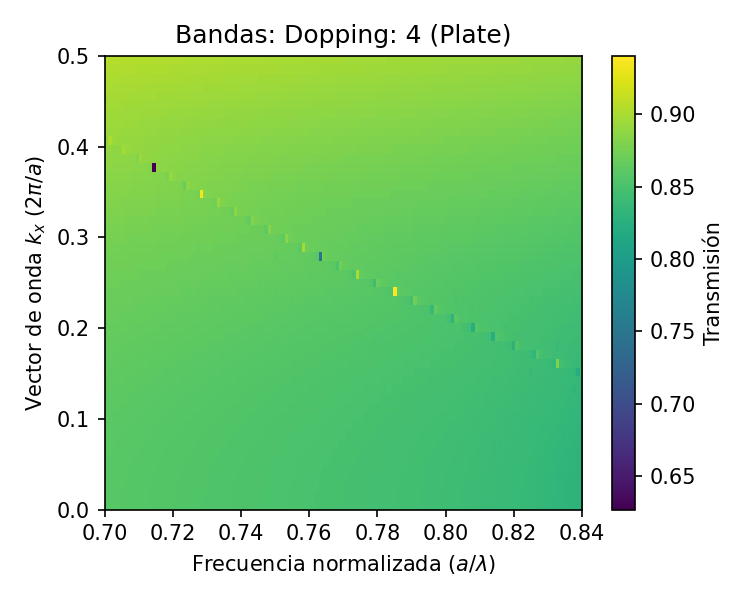
\includegraphics[width=0.48\textwidth]{figures/Dopping: 4_plate.png}
\hfill
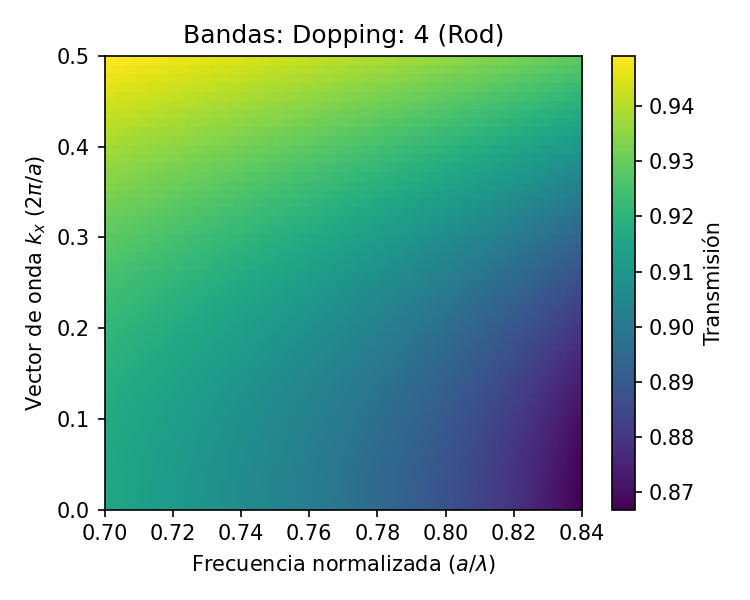
\includegraphics[width=0.48\textwidth]{figures/Dopping: 4_rod.png}
\caption{Estructuras de bandas fotónicas ($k_x$) para Dopping: 4. Izquierda: Lámina. Derecha: Cilindros.}
\end{figure}
\vspace{1em}
\begin{figure}[H]
\centering
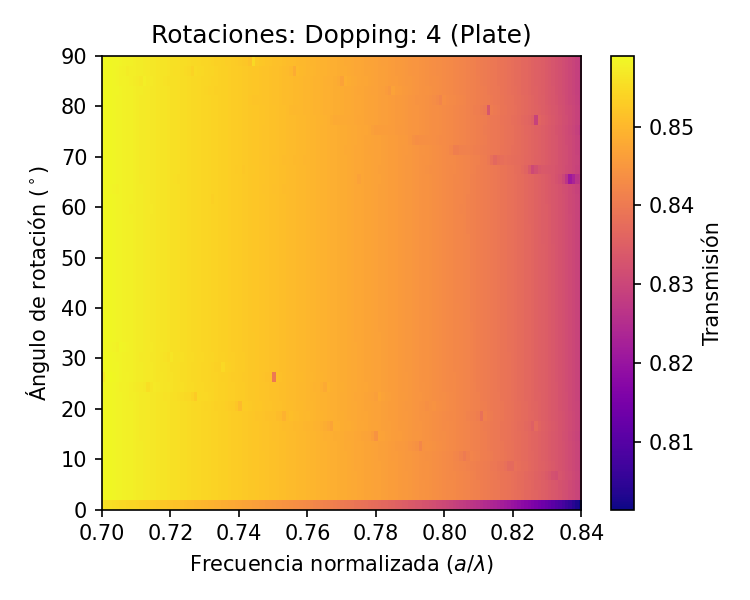
\includegraphics[width=0.48\textwidth]{figures/Dopping: 4_plate_rangle.png}
\hfill
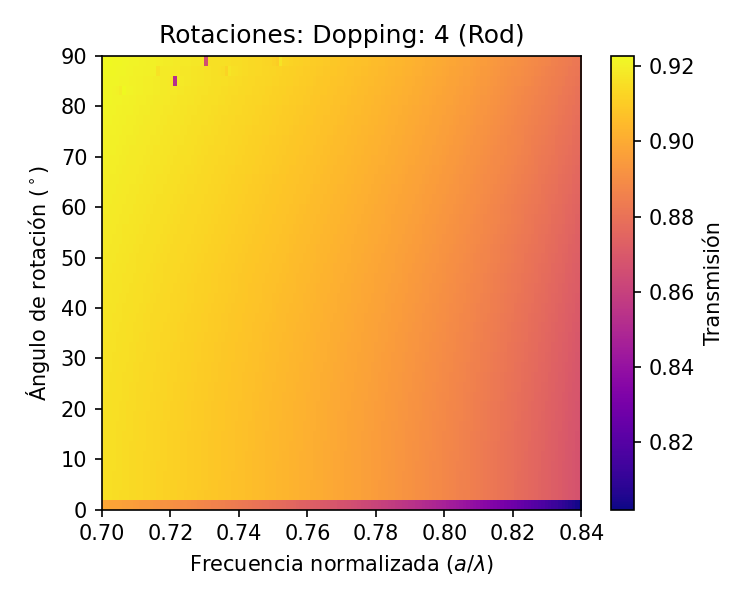
\includegraphics[width=0.48\textwidth]{figures/Dopping: 4_rod_rangle.png}
\caption{Mapas de transmisión por rotación (twist) para Dopping: 4. Izquierda: Lámina. Derecha: Cilindros.}
\end{figure}
\vspace{1em}
\hrule
\vspace{1em}
\subsection*{Material ID: Dopping: 8}
\textbf{Constante Dieléctrica ($\epsilon_{total}$):} 2.65 \\[0.5em]
\begin{table}[h!]
\centering
\begin{tabular}{lcc}
\toprule
\textbf{Métrica} & \textbf{Lámina (Plate)} & \textbf{Cilindros (Rod)} \\
\midrule
Bandgaps ($k_x$) & Ninguno & Ninguno \\
Resonancias ($k_x$) & 36 & 36 \\
\midrule
Bandgaps (Rotación) & Ninguno & Ninguno \\
Resonancias (Rotación) & 33 & 33 \\
\bottomrule
\end{tabular}
\end{table}
\begin{figure}[H]
\centering
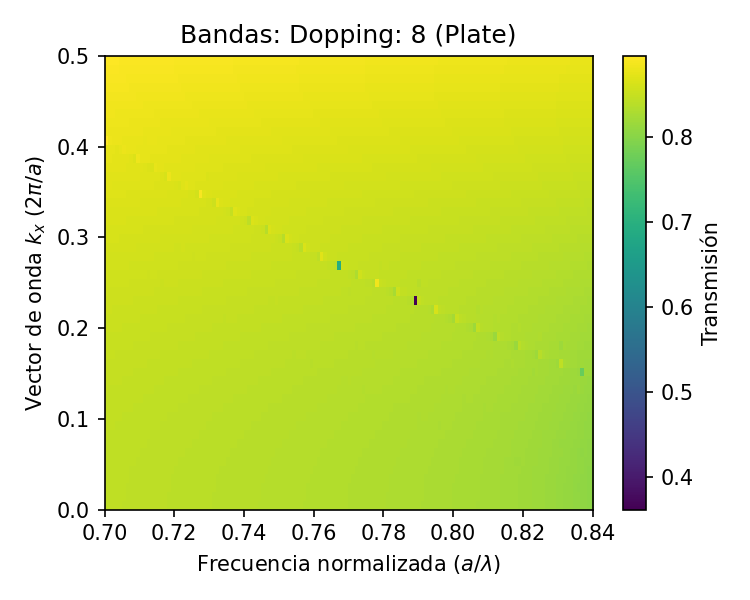
\includegraphics[width=0.48\textwidth]{figures/Dopping: 8_plate.png}
\hfill
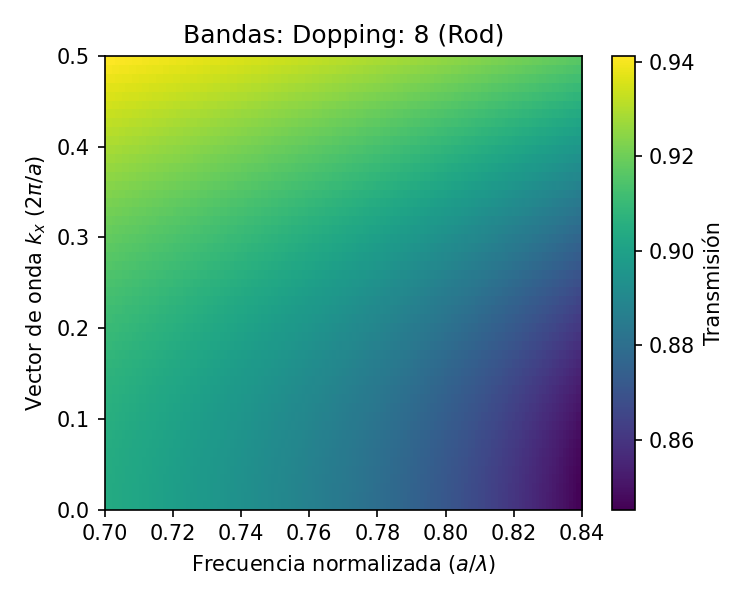
\includegraphics[width=0.48\textwidth]{figures/Dopping: 8_rod.png}
\caption{Estructuras de bandas fotónicas ($k_x$) para Dopping: 8. Izquierda: Lámina. Derecha: Cilindros.}
\end{figure}
\vspace{1em}
\begin{figure}[H]
\centering
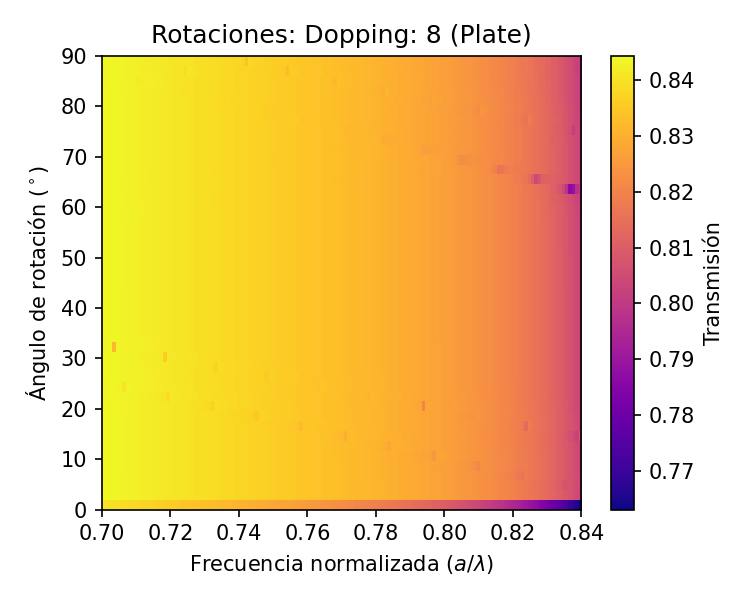
\includegraphics[width=0.48\textwidth]{figures/Dopping: 8_plate_rangle.png}
\hfill
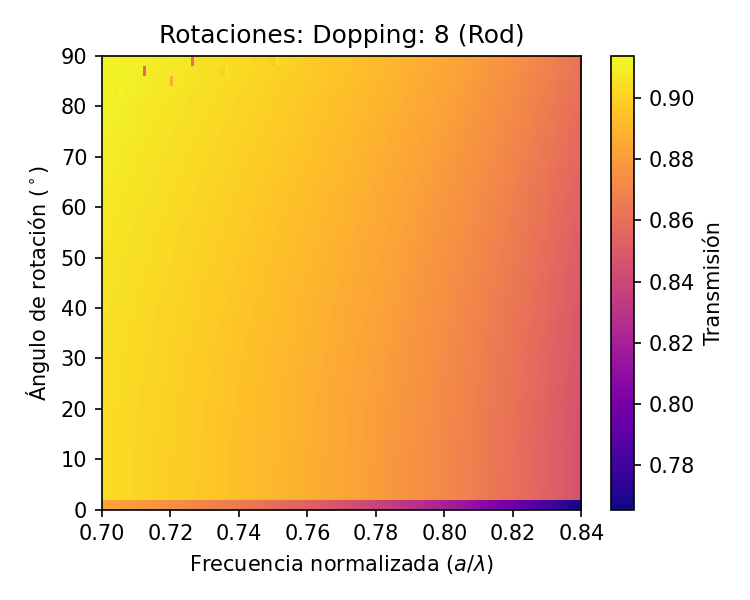
\includegraphics[width=0.48\textwidth]{figures/Dopping: 8_rod_rangle.png}
\caption{Mapas de transmisión por rotación (twist) para Dopping: 8. Izquierda: Lámina. Derecha: Cilindros.}
\end{figure}
\vspace{1em}
\hrule
\vspace{1em}
\clearpage
\section{PMMA without doping}
\subsection*{Material ID: Thickness: 100}
\textbf{Constante Dieléctrica ($\epsilon_{total}$):} 2.52 \\[0.5em]
\begin{table}[h!]
\centering
\begin{tabular}{lcc}
\toprule
\textbf{Métrica} & \textbf{Lámina (Plate)} & \textbf{Cilindros (Rod)} \\
\midrule
Bandgaps ($k_x$) & Ninguno & Ninguno \\
Resonancias ($k_x$) & 36 & 36 \\
\midrule
Bandgaps (Rotación) & Ninguno & Ninguno \\
Resonancias (Rotación) & 33 & 33 \\
\bottomrule
\end{tabular}
\end{table}
\begin{figure}[H]
\centering
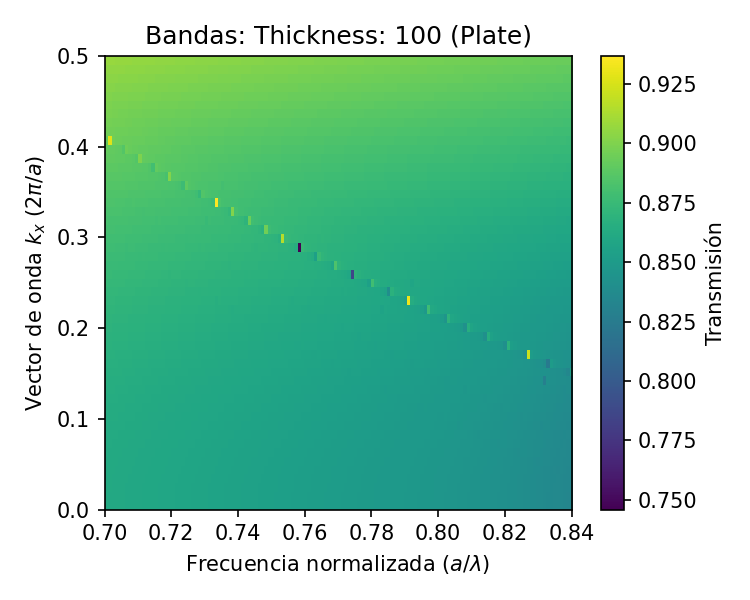
\includegraphics[width=0.48\textwidth]{figures/Thickness: 100_plate.png}
\hfill
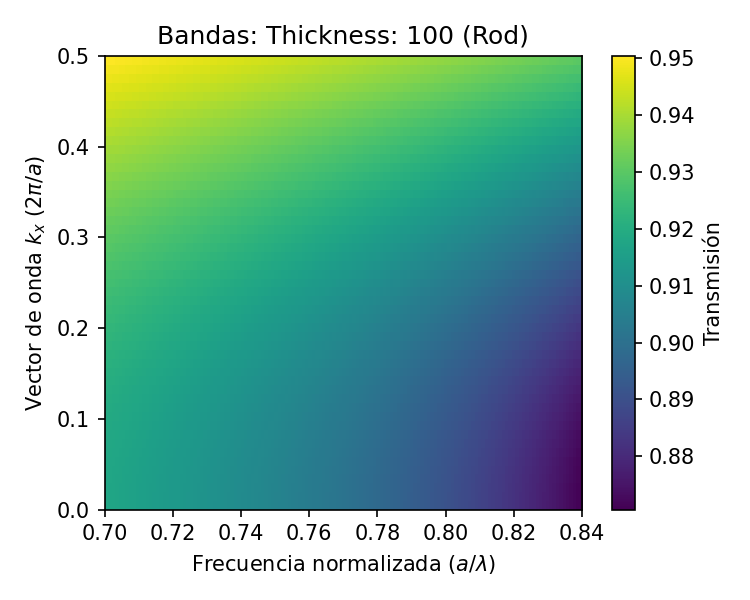
\includegraphics[width=0.48\textwidth]{figures/Thickness: 100_rod.png}
\caption{Estructuras de bandas fotónicas ($k_x$) para Thickness: 100. Izquierda: Lámina. Derecha: Cilindros.}
\end{figure}
\vspace{1em}
\begin{figure}[H]
\centering
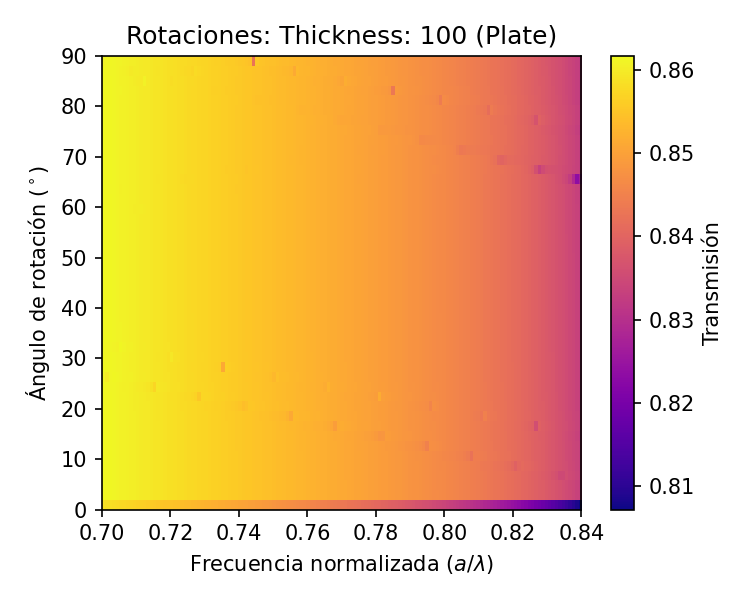
\includegraphics[width=0.48\textwidth]{figures/Thickness: 100_plate_rangle.png}
\hfill
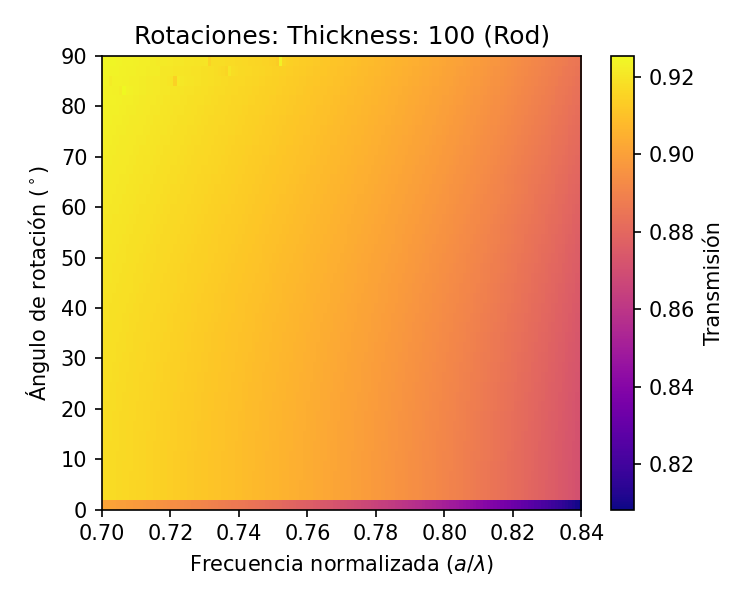
\includegraphics[width=0.48\textwidth]{figures/Thickness: 100_rod_rangle.png}
\caption{Mapas de transmisión por rotación (twist) para Thickness: 100. Izquierda: Lámina. Derecha: Cilindros.}
\end{figure}
\vspace{1em}
\hrule
\vspace{1em}
\subsection*{Material ID: Thickness: 150}
\textbf{Constante Dieléctrica ($\epsilon_{total}$):} 2.53 \\[0.5em]
\begin{table}[h!]
\centering
\begin{tabular}{lcc}
\toprule
\textbf{Métrica} & \textbf{Lámina (Plate)} & \textbf{Cilindros (Rod)} \\
\midrule
Bandgaps ($k_x$) & Ninguno & Ninguno \\
Resonancias ($k_x$) & 36 & 36 \\
\midrule
Bandgaps (Rotación) & Ninguno & Ninguno \\
Resonancias (Rotación) & 33 & 33 \\
\bottomrule
\end{tabular}
\end{table}
\begin{figure}[H]
\centering
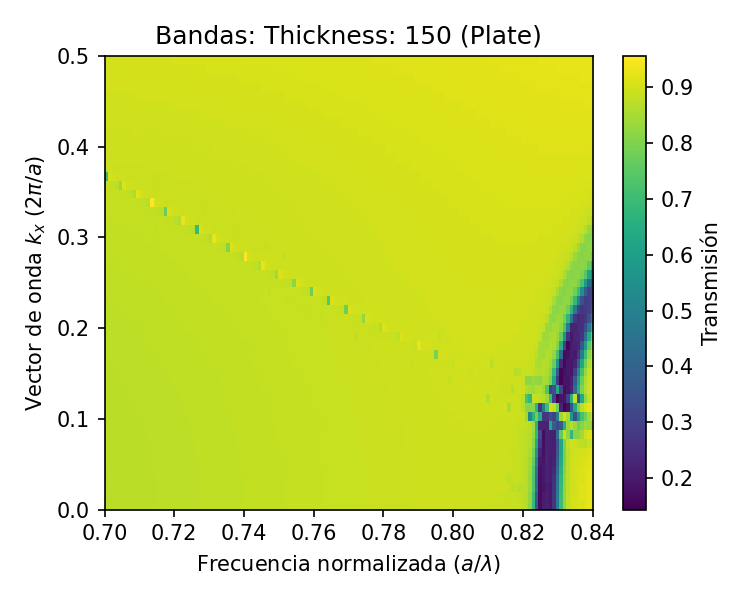
\includegraphics[width=0.48\textwidth]{figures/Thickness: 150_plate.png}
\hfill
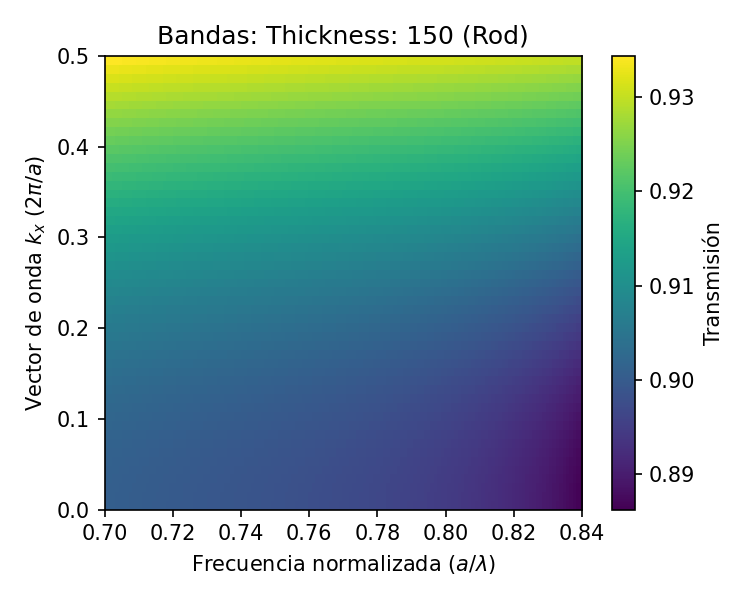
\includegraphics[width=0.48\textwidth]{figures/Thickness: 150_rod.png}
\caption{Estructuras de bandas fotónicas ($k_x$) para Thickness: 150. Izquierda: Lámina. Derecha: Cilindros.}
\end{figure}
\vspace{1em}
\begin{figure}[H]
\centering
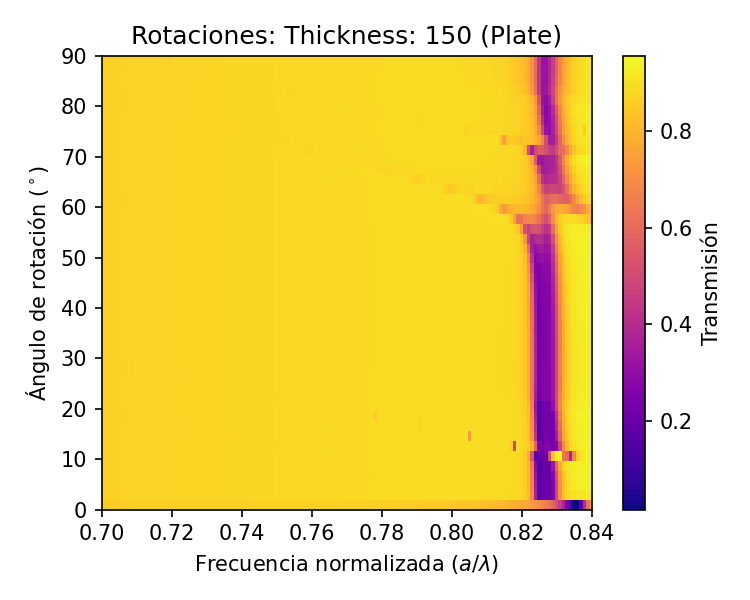
\includegraphics[width=0.48\textwidth]{figures/Thickness: 150_plate_rangle.png}
\hfill
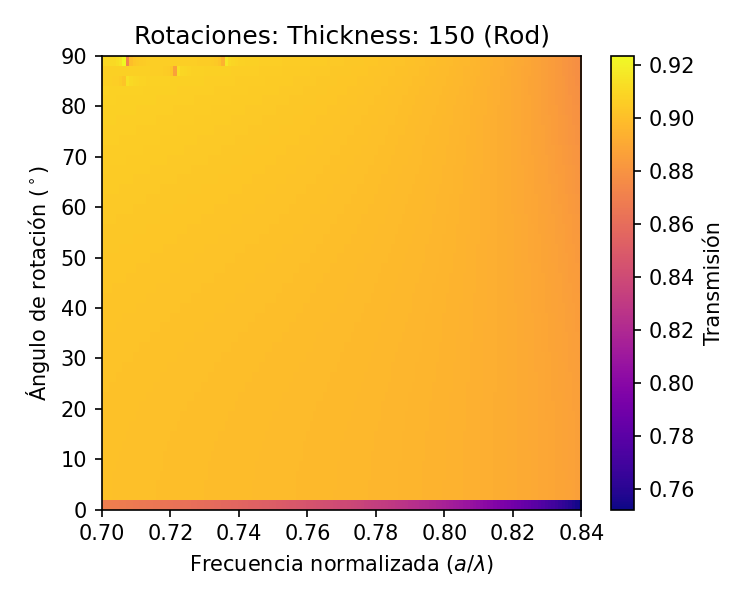
\includegraphics[width=0.48\textwidth]{figures/Thickness: 150_rod_rangle.png}
\caption{Mapas de transmisión por rotación (twist) para Thickness: 150. Izquierda: Lámina. Derecha: Cilindros.}
\end{figure}
\vspace{1em}
\hrule
\vspace{1em}
\subsection*{Material ID: Thickness: 200}
\textbf{Constante Dieléctrica ($\epsilon_{total}$):} 2.47 \\[0.5em]
\begin{table}[h!]
\centering
\begin{tabular}{lcc}
\toprule
\textbf{Métrica} & \textbf{Lámina (Plate)} & \textbf{Cilindros (Rod)} \\
\midrule
Bandgaps ($k_x$) & Ninguno & Ninguno \\
Resonancias ($k_x$) & 36 & 36 \\
\midrule
Bandgaps (Rotación) & Ninguno & Ninguno \\
Resonancias (Rotación) & 33 & 33 \\
\bottomrule
\end{tabular}
\end{table}
\begin{figure}[H]
\centering
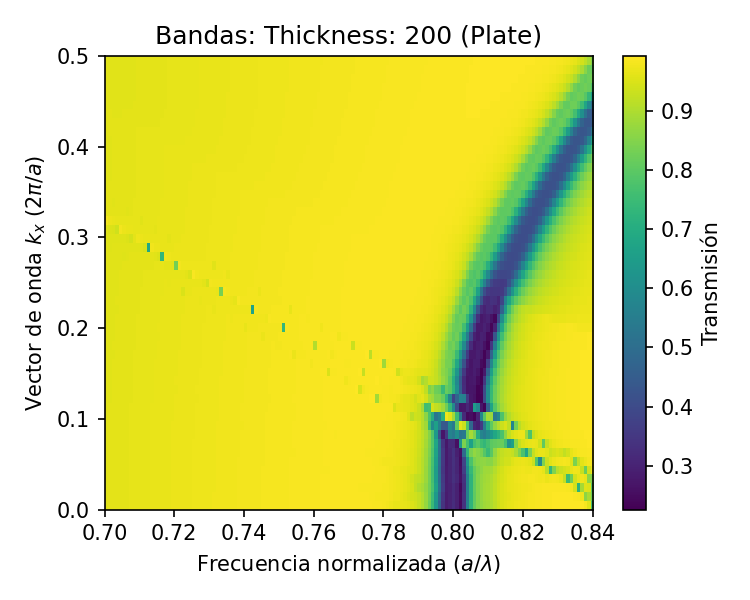
\includegraphics[width=0.48\textwidth]{figures/Thickness: 200_plate.png}
\hfill
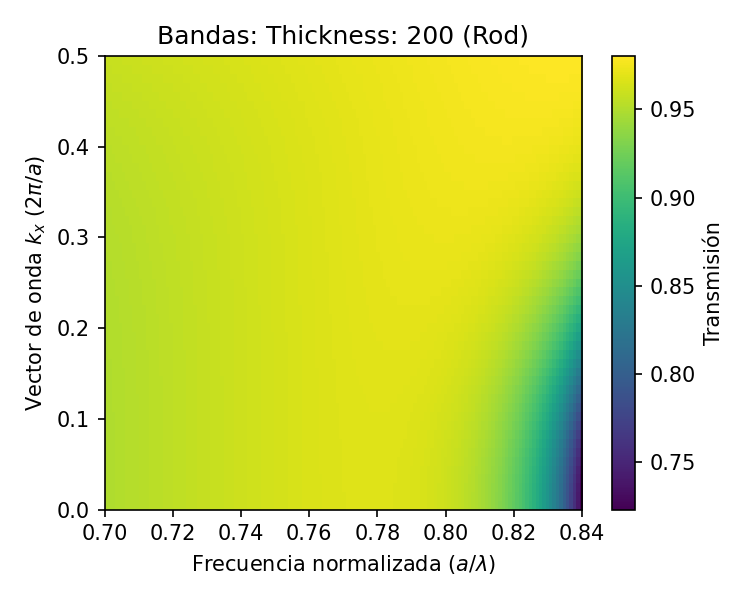
\includegraphics[width=0.48\textwidth]{figures/Thickness: 200_rod.png}
\caption{Estructuras de bandas fotónicas ($k_x$) para Thickness: 200. Izquierda: Lámina. Derecha: Cilindros.}
\end{figure}
\vspace{1em}
\begin{figure}[H]
\centering
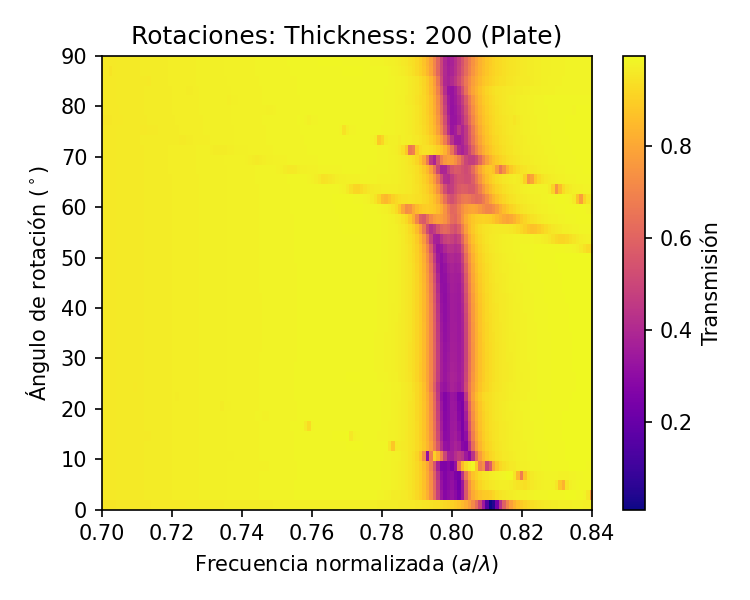
\includegraphics[width=0.48\textwidth]{figures/Thickness: 200_plate_rangle.png}
\hfill
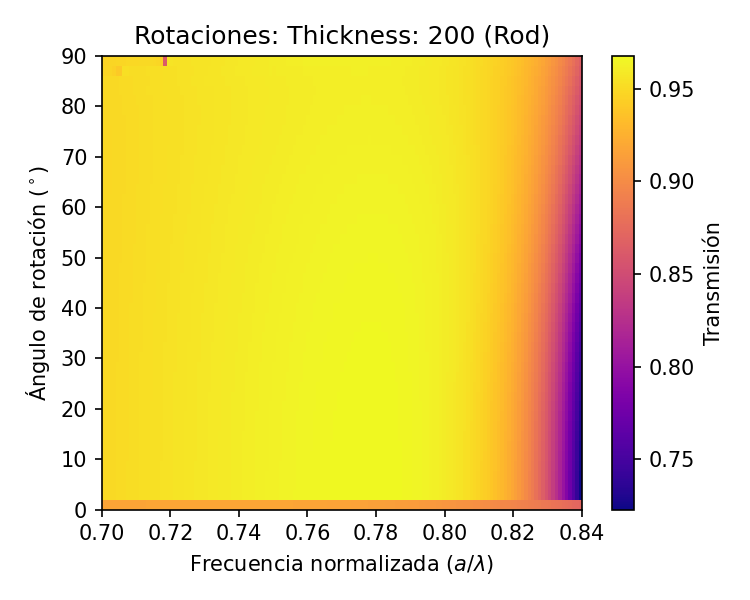
\includegraphics[width=0.48\textwidth]{figures/Thickness: 200_rod_rangle.png}
\caption{Mapas de transmisión por rotación (twist) para Thickness: 200. Izquierda: Lámina. Derecha: Cilindros.}
\end{figure}
\vspace{1em}
\hrule
\vspace{1em}
\subsection*{Material ID: Thickness: 60}
\textbf{Constante Dieléctrica ($\epsilon_{total}$):} 2.67 \\[0.5em]
\begin{table}[h!]
\centering
\begin{tabular}{lcc}
\toprule
\textbf{Métrica} & \textbf{Lámina (Plate)} & \textbf{Cilindros (Rod)} \\
\midrule
Bandgaps ($k_x$) & Ninguno & Ninguno \\
Resonancias ($k_x$) & 36 & 36 \\
\midrule
Bandgaps (Rotación) & Ninguno & Ninguno \\
Resonancias (Rotación) & 33 & 33 \\
\bottomrule
\end{tabular}
\end{table}
\begin{figure}[H]
\centering
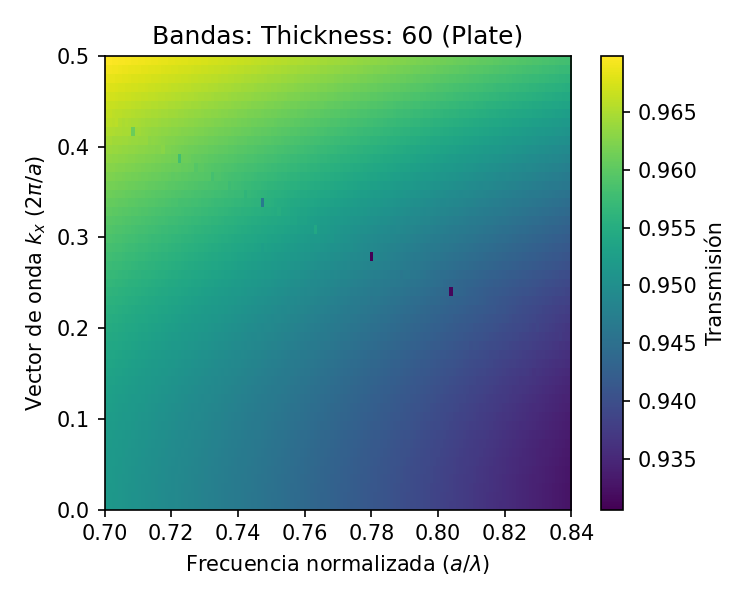
\includegraphics[width=0.48\textwidth]{figures/Thickness: 60_plate.png}
\hfill
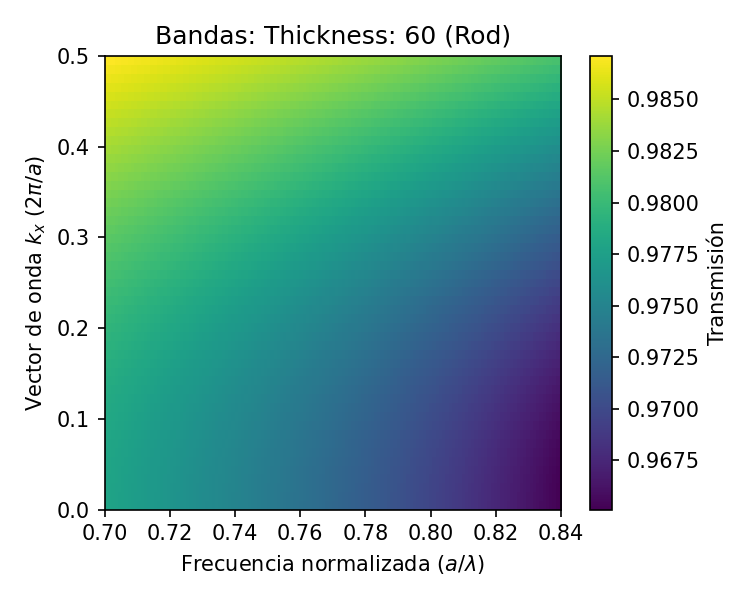
\includegraphics[width=0.48\textwidth]{figures/Thickness: 60_rod.png}
\caption{Estructuras de bandas fotónicas ($k_x$) para Thickness: 60. Izquierda: Lámina. Derecha: Cilindros.}
\end{figure}
\vspace{1em}
\begin{figure}[H]
\centering
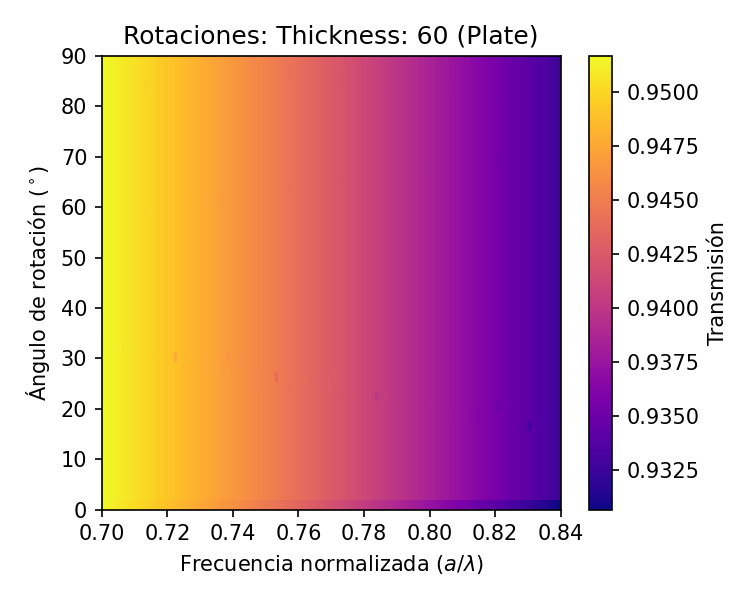
\includegraphics[width=0.48\textwidth]{figures/Thickness: 60_plate_rangle.png}
\hfill
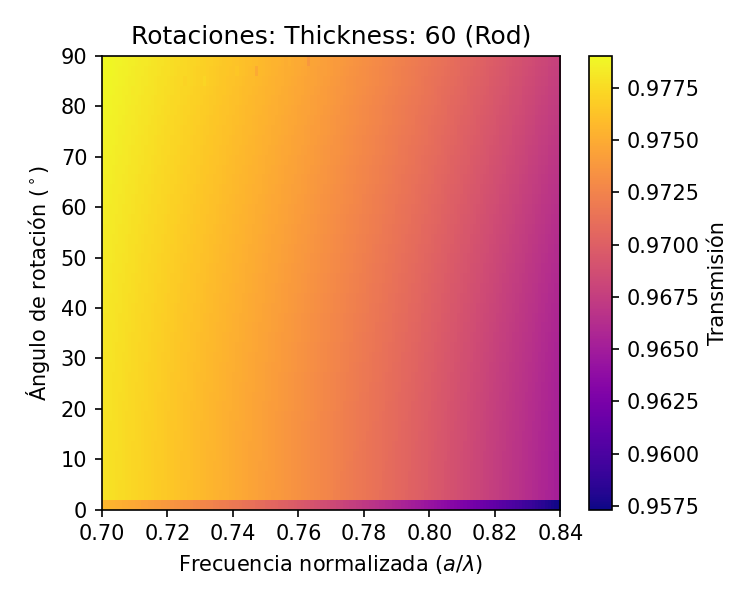
\includegraphics[width=0.48\textwidth]{figures/Thickness: 60_rod_rangle.png}
\caption{Mapas de transmisión por rotación (twist) para Thickness: 60. Izquierda: Lámina. Derecha: Cilindros.}
\end{figure}
\vspace{1em}
\hrule
\vspace{1em}
\clearpage
\end{document}